%**************************************************************
%%**************************************************************
\documentclass[%
	pdftex,
	oneside,			% Einseitiger Druck.
	12pt,				% Schriftgroesse
	parskip=half,		% Halbe Zeile Abstand zwischen Absätzen.
	headsepline,		% Linie nach Kopfzeile.
	footsepline,		% Linie vor Fusszeile.
	abstract=true,		% Abstract Überschriften
	ngerman,			% Translator
]{scrreprt}

%!TEX root = ../dokumentation.tex

%
% Nahezu alle Einstellungen koennen hier getaetigt werden
%

% Zeichencodierung
\usepackage[utf8]{inputenc}
\usepackage[T1]{fontenc}
\usepackage{lmodern}
\usepackage[official]{eurosym}

% Zeilenabstand
\usepackage[onehalfspacing]{setspace}


% Seitenränder anpassen 
%\usepackage[paper=a4paper,left=2.5cm,right=2.5cm,top=2.5cm,bottom=2.5cm]{geometry}
\usepackage{geometry}
\setlength{\topskip}{\ht\strutbox} % behebt Warnung von geometry 
\setlength{\headheight}{1.1\baselineskip}   % Headheight hochsetzten 
\renewcommand*{\chapterheadstartvskip}{\vspace*{.5\baselineskip}}% Abstand einstellen

%PDF als ganze Seite einbinden
\usepackage{pdfpages}

%Seitengroesse
\usepackage{fullpage}

%Zeilenumbruch und mehr
\usepackage[activate]{microtype}

% gestrichelte Linien
\usepackage{dashrule}

% Index-Erstellung
\usepackage{makeidx}

% Lokalisierung (neue deutsche Rechtschreibung)
\usepackage[ngerman]{babel}

% Anführungszeichen 
\usepackage[babel,german=quotes]{csquotes}

% Grafiken
\usepackage{graphicx}
\usepackage{subfig}
\usepackage{caption}
\DeclareCaptionLabelFormat{blank}{}
%\usepackage{subcaption}
\usepackage{float}
\restylefloat{figure}

% Mathematische Textsaetze
\usepackage{amsmath}
\usepackage{amssymb}

%checkmarks
\usepackage{pifont}
\newcommand{\cmark}{\ding{51}}%
\newcommand{\xmark}{\ding{55}}%
%footnotes in a table
\usepackage{setspace}
\usepackage{threeparttable}

% Farben
\usepackage{color}
\definecolor{LinkColor}{rgb}{0,0,0.2}
\definecolor{ListingBackground}{rgb}{0.92,0.92,0.92}

% PDF Einstellungen
\usepackage{hyperref}
[%
	%pdftitle={\pdftitel},
	%pdfauthor={\autor},
	%pdfsubject={\arbeit},
	pdfcreator={pdflatex, LaTeX with KOMA-Script},
	pdfpagemode=UseOutlines, % Beim Oeffnen Inhaltsverzeichnis anzeigen
	pdfdisplaydoctitle=true, % Dokumenttitel statt Dateiname anzeigen.
	pdflang=de % Sprache des Dokuments.
]

% (Farb-)einstellungen für die Links im PDF
\hypersetup{%
	colorlinks=true, % Aktivieren von farbigen Links im Dokument
	linkcolor=black, % Farbe festlegen
	citecolor=black,
	filecolor=LinkColor,
	menucolor=LinkColor,
	urlcolor=black,  %%changed to black	
	bookmarksnumbered=true % Überschriftsnummerierung im PDF Inhalt anzeigen.
}

% Literaturverweise 
\usepackage[authoryear]{natbib}
\newcommand{\literaturverz}[1]{
	%Autorenverknüpfung mit "und"
	\renewcommand{\harvardand}{and}
	\bibliography{#1}
}

% http://projekte.dante.de/DanteFAQ/Silbentrennung
\usepackage{microtype}
\clubpenalty=10000
\widowpenalty=10000
\displaywidowpenalty=10000

% Quellcode

\usepackage{listings} % Einbinden des Listings-Pakets für Code-Listings

% Definition von benutzerdefinierten Farben
\definecolor{KeywordPurple}{rgb}{0.5, 0.0, 0.5}
\definecolor{CommentGreen}{rgb}{0.13, 0.55, 0.13}
\definecolor{StringOrange}{rgb}{0.8, 0.33, 0.0}
\definecolor{TypeBlue}{rgb}{0.2, 0.2, 0.8} % Sanfteres Blau
\definecolor{IntMagenta}{rgb}{0.8, 0.2, 0.8} % Sanfteres Magenta
\definecolor{ClassGreen}{rgb}{0.0, 0.75, 0.5} % Türkis, weniger grell
\definecolor{FunctionsYellow}{rgb}{0.9, 0.8, 0.1} % Weniger grelles Gelb
% Definition eines benutzerdefinierten JSON-Sprachstils
\lstdefinelanguage{json}{
    morestring=[b]",                % Definiert das Anführungszeichen als String-Begrenzer
    stringstyle=\color{CommentGreen},    % Setzt die Farbe der Strings auf Grün
    literate=                       % Ermöglicht die Formatierung einzelner Zeichen oder Zeichenfolgen
     *{0}{{{\color{IntMagenta}0}}}{1}
      {1}{{{\color{IntMagenta}1}}}{1}
      {2}{{{\color{IntMagenta}2}}}{1}
      {3}{{{\color{IntMagenta}3}}}{1}
      {4}{{{\color{IntMagenta}4}}}{1}
      {5}{{{\color{IntMagenta}5}}}{1}
      {6}{{{\color{IntMagenta}6}}}{1}
      {7}{{{\color{IntMagenta}7}}}{1}
      {8}{{{\color{IntMagenta}8}}}{1}
      {9}{{{\color{IntMagenta}9}}}{1}
      {"Test}{{{\color{StringOrange}"Test}}}{4}
      {ID"}{{{\color{StringOrange}ID"}}}{2}
      {Description"}{{{\color{StringOrange}Description"}}}{10}
      {"..//"}{{{\color{StringOrange}"..//"}}}{4},
}

% Definition eines benutzerdefinierten JSON-Stils
\lstdefinestyle{myJSON}{
	backgroundcolor=\color{white},   % Setzt die Hintergrundfarbe auf Weiß
	basicstyle=\scriptsize\ttfamily, % Setzt die Basis-Schriftart und -größe
	breaklines=true,                 % Ermöglicht das Umbruch von langen Zeilen
	captionpos=b,                    % Position der Beschriftung unterhalb des Listings
	frame=single,                    % Rahmenart: einfacher Rahmen um das Listing
	keepspaces=true,                 % Beibehalten von Leerzeichen im Code, nützlich für die Einrückung
	language=json,                   % Setzt die Sprache des Listings auf JSON
	numbers=left,                    % Zeilennummern auf der linken Seite
	numbersep=5pt,                   % Abstand der Zeilennummern zum Text
	numberstyle=\scriptsize,         % Stil und Größe der Zeilennummern
	rulecolor=\color{black},         % Farbe des Rahmens
	showstringspaces=false,          % Keine speziellen Markierungen für Leerzeichen in Strings
	tabsize=2,                       % Größe eines Tabulators ist 2 Leerzeichen
	keywordstyle=[2]\color{TypeBlue},    % Farbe der Schlüsselwörter (true, false) auf Blau setzen
	keywords=[2]{true, false}        % Definiert zusätzliche Schlüsselwörter
}

\lstloadlanguages{C++}

% Definition eines benutzerdefinierten C++-Stils
\lstdefinestyle{myCPP}{
	backgroundcolor=\color{white},
	basicstyle=\scriptsize\ttfamily,
	breaklines=true,
	breakindent=20pt,
	% breakatwhitespace=true, 
	postbreak=\mbox{\textcolor{gray}{$\hookrightarrow$}\space},
	captionpos=b,
	frame=single,
	keepspaces=true,
	language=C++,
	numbers=left,
	numbersep=5pt,
	numberstyle=\scriptsize,
	rulecolor=\color{black},
	showstringspaces=false,
	tabsize=2,
	stringstyle=\color{StringOrange},
	commentstyle=\color{CommentGreen},
	morekeywords={string, time_t, size_t, curl_easy_setopt},
	keywordstyle=\color{TypeBlue},
	emph={using, return, if, else, switch, case, break},
	emphstyle=\color{KeywordPurple},
	emph={[2]std, chrono, stringstream, system_clock, helper, RequestProvider, shared_ptr, mvIMPACT, acquire, ImageBuffer, this_thread, filesystem, milliseconds, ImpactAcquireException, spdlog, ifstream, nlohmann, level, DeviceManager, termios, json, CURL, CURLcode, ConfigurationParameter, ThreadParameter, Device, exception, Statistics, TimestampProvider, ConfigurationHandler, ImageSavePreparer, Logger, AzureIssueCreator},
	emphstyle={[2]\color{ClassGreen}},
	emph={[3]getTimestamp, str, localtime, put_time, processRequest, isOK, duration_cast, getDeviceFromUserInput, sleep_for, acquisitionStop, open, parse, getBufferPart, getErrorCodeAsString, acquisitionStart, reset, ref, getImageBufferDesc, getBuffer, save, now, basic_logger_mt, curl_slist_free_all, curl_easy_cleanup, tcgetattr, fcntl, getchar, ungetc, base64_encode, curl_easy_init, curl_slist_append, curl_easy_perform, curl_easy_strerror, create_directories, ceil, name, readS, read, append, to_string, mkdir, set_level, set_pattern, rotating_logger_mt, flush_on, c_str, time_since_epoch, setfill, setw, is_string, is_boolean, is_number_integer, count, get, empty, isalnum, to_time_t, getTimestamp_ms, getNowTime, operator=, loadConfiguration, checkPath, createFolder, readConfigurationParameter, checkConfigurationParameter, createOutputDirectories, prepareImageSave, prepareBufferSave, createImageSubpathFolder, createBufferSubpathFolder, initializeLogger, logStatistics, setLogLevel, interpretStatistics, sendAzureIssue, checkKeyboardHit, createAzureIssue, handleCurlResponse},
	emphstyle={[3]\color{FunctionsYellow}},
	escapeinside={@@},
	literate=
		{0}{{\textcolor{IntMagenta}{0}}}1
		{1}{{\textcolor{IntMagenta}{1}}}1
		{2}{{\textcolor{IntMagenta}{2}}}1
		{3}{{\textcolor{IntMagenta}{3}}}1
		{4}{{\textcolor{IntMagenta}{4}}}1
		{5}{{\textcolor{IntMagenta}{5}}}1
		{6}{{\textcolor{IntMagenta}{6}}}1
		{7}{{\textcolor{IntMagenta}{7}}}1
		{8}{{\textcolor{IntMagenta}{8}}}1
		{9}{{\textcolor{IntMagenta}{9}}}1
}


\lstdefinestyle{myHPP}{
	backgroundcolor=\color{white},
	basicstyle=\scriptsize\ttfamily,
	breaklines=true,
	breakindent=20pt,
	breakatwhitespace=true, 
	postbreak=\mbox{\textcolor{gray}{$\hookrightarrow$}\space},
	captionpos=b,
	frame=single,
	keepspaces=true,
	language=C++,
	numbers=left,
	numbersep=5pt,
	numberstyle=\scriptsize,
	rulecolor=\color{black},
	showstringspaces=false,
	tabsize=2,
	stringstyle=\color{StringOrange},
	moredelim=[s][\color{StringOrange}]{<}{>},
	commentstyle=\color{CommentGreen},
	morekeywords={string, time_t, size_t},
	keywordstyle=\color{TypeBlue},
	emph={using},
	emphstyle=\color{KeywordPurple},
	emph={[2]std, ConfigurationParameter, ThreadParameter, Device, Statistics, TimestampProvider, ConfigurationHandler, ImageSavePreparer, Logger, AzureIssueCreator},
	emphstyle={[2]\color{ClassGreen}},
	emph={[3]getTimestamp, getTimestamp_ms, getNowTime, operator=, loadConfiguration, checkPath, createFolder, readConfigurationParameter, checkConfigurationParameter, createOutputDirectories, prepareImageSave, prepareBufferSave, createImageSubpathFolder, createBufferSubpathFolder, initializeLogger, logStatistics, setLogLevel, interpretStatistics, sendAzureIssue, checkKeyboardHit, createAzureIssue, handleCurlResponse},
	emphstyle={[3]\color{FunctionsYellow}},
	escapeinside={@@},
	literate=
		{0}{{\textcolor{IntMagenta}{0}}}1
		{1}{{\textcolor{IntMagenta}{1}}}1
		{2}{{\textcolor{IntMagenta}{2}}}1
		{3}{{\textcolor{IntMagenta}{3}}}1
		{4}{{\textcolor{IntMagenta}{4}}}1
		{5}{{\textcolor{IntMagenta}{5}}}1
		{6}{{\textcolor{IntMagenta}{6}}}1
		{7}{{\textcolor{IntMagenta}{7}}}1
		{8}{{\textcolor{IntMagenta}{8}}}1
		{9}{{\textcolor{IntMagenta}{9}}}1
}

% Glossar
\usepackage[
	nonumberlist, %keine Seitenzahlen anzeigen
	acronym,      %ein Abkürzungsverzeichnis erstellen
	%section,     %im Inhaltsverzeichnis auf section-Ebene erscheinen
	toc,          %Einträge im Inhaltsverzeichnis
]{glossaries}

%Abkürzungsverzeichnis
\usepackage[nohyperlinks]{acronym}

%Bildpfad
\graphicspath{{images/}}

%nur ein latex-Durchlauf für die Aktualisierung von Verzeichnissen nötig
\usepackage{bookmark}

% eine Kommentarumgebung "k" (Handhabe mit \begin{k}<Kommentartext>\end{k},
% Kommentare werden rot gedruckt). Wird \% vor excludecomment{k} entfernt,
% werden keine Kommentare mehr gedruckt.
\usepackage{comment}
\specialcomment{k}{\begingroup\color{red}}{\endgroup}
%\excludecomment{k}

%Color in tables
\usepackage{colortbl}
	% Ab jetzt können auch Umlaute verwendet werden

\makeglossaries{}
%!TEX root = ../dokumentation.tex

%
% vorher in Konsole folgendes aufrufen: 
% makeglossaries makeglossaries dokumentation.acn && makeglossaries dokumentation.glo
%

%
% Glossareintraege --> referenz, name, beschreibung
% Aufruf mit \gls{...}
%

\newglossaryentry{Glossareintrag}{name={Glossareintrag},plural={Glossareinträge},description={Ein Glossar beschreibt verschiedenste Dinge in kurzen Worten}}

\begin{document}
\hypersetup{linkcolor=black} 
	% Deckblatt
	%!TEX root = ../dokumentation.tex

\newcommand{\kurzerUnterstrich}{\rule[-1pt]{5pt}{0.5pt}}

\begin{titlepage}
	\begin{center}
		\begin{longtable}{@{}>{\raggedright}p{.5\linewidth}@{}>{\raggedleft}p{.5\linewidth}@{}}
			
\includegraphics[width=7cm]{images/BALLUFF.png} & 
			
\includegraphics[width=5cm]{images/DHBW.png}
		\end{longtable}
	\end{center}
	\enlargethispage{12mm}
	\begin{center}
						{\Large {Entwicklung und Implementierung eines Testkonzepts}}\\
		\vspace*{3mm}	{\Large {für die Datenauswertung des RadarImagers unter}}\\
		\vspace*{3mm}	{\Large {Verwendung von C++}}\\
		\vspace*{12mm}	{\large\textbf {T2000\kurzerUnterstrich02}} \\
		\vspace*{12mm}	{für die Prüfung zum}\\
		\vspace*{3mm}	{\textbf {Bachelor of Engineering}}\\
		\vspace*{12mm}	{des Studiengangs Elektrotechnik - Elektronik}\\
    	\vspace*{3mm}	{an der Dualen Hochschule Baden-Württemberg Stuttgart}\\
		\vspace*{12mm}	{von}\\
		\vspace*{3mm}	{\large\textbf {Nico Durst-Claus}}\\
		\vspace*{12mm}	{02. September 2024}\\
	\end{center}
	\vfill
	\begin{spacing}{1.2}
	\begin{tabbing}
		mmmmmmmmmmmmmmmmmmmmmmmmmmmm					\= \kill
		\textbf{Bearbeitungszeitraum}                   \>  27.05.2024 - 02.09.2024\\
		\textbf{Matrikelnummer}                         \>  7199590\\
		\textbf{Kurs}                                   \>  TEL22GR2\\
		\textbf{Ausbildungsunternehmen}                 \>  Balluff GmbH, Neuhausen a.d.F.\\
		\textbf{Betreuer des Ausbildungsunternehmens}   \>  Patrick Benz (B. Eng.)\\
	\end{tabbing}
	\end{spacing}
\end{titlepage}
	
	\newpage
	
	% Erklärung
	%!TEX root = ../dokumentation.tex

\thispagestyle{empty}

\section*{Eidesstattliche Erklärung}

Ich versichere hiermit, dass ich meine Projektarbeit mit dem Thema:
\begin{center}
    \glqq Entwicklung und Implementierung eines Testkonzepts für die\\ 
    Datenauswertung des RadarImagers unter Verwendung von C++\grqq
\end{center}
selbstständig verfasst und keine anderen als die angegebenen Quellen und Hilfsmittel benutzt habe. Ich versichere zudem, dass die eingereichte elektronische Fassung mit der gedruckten Fassung übereinstimmt.

\vspace*{3mm}

\begin{center}
    \begin{tabular*}{15cm}{@{\extracolsep{\fill}}>{\centering\arraybackslash}p{7.5cm}>{\centering\arraybackslash}p{7.5cm}@{}}
        \hdashrule{6cm}{1pt}{1mm} & \hdashrule{6cm}{1pt}{1mm}\\
        Ort, Datum & Unterschrift\ 
    \end{tabular*}
\end{center}

\vfill

\section*{Gender-Hinweis}

Aus Gründen der Lesbarkeit wird in dieser Projektarbeit darauf verzichtet, durchgehend geschlechterspezifische Formulierungen zu verwenden. Soweit personenbezogene Bezeichnungen nur in männlicher Form angeführt sind, beziehen sie sich auf Männer, Frauen und Diverse 
in gleicher Weise.\\
Dies soll jedoch keinesfalls eine Geschlechterdiskriminierung oder eine Verletzung des Gleichheitsgrundsatzes zum Ausdruck bringen. Entsprechende Begriffe gelten im Sinne der Gleichbehandlung grundsätzlich für alle Geschlechter. Die verkürzte Sprachform beinhaltet keine 
Wertung.

\cleardoubleemptypage



	\newpage
	%Sperrvermerk
	\thispagestyle{empty}

\section*{Sperrvermerk}

Die gesamte Arbeit ist geistiges Eigentum des Verfassers und der Balluff GmbH. Die verwendeten Zitate und Abbildungen anderer Autoren sind als deren geistiges Eigentum durch das Copyright ebenfalls geschützt. Eine Verwendung dieser Arbeit, auch nur in Auszügen ist, ohne ausdrückliche Genehmigung des Verfassers und der Balluff GmbH, rechtswidrig.

\begin{center}
    \textsuperscript{\textcopyright}\\
    Nico Durst-Claus\\
    Balluff GmbH\\
\end{center}

\cleardoubleemptypage{}
	
	% Abstract
	%!TEX root = ../dokumentation.tex

\thispagestyle{empty}

\section*{Zusammenfassung}
 
Hier steht die deutsche Zusammenfassung

\cleardoubleemptypage{}

\newpage

\thispagestyle{empty}

\section*{Abstract}

Hier steht die englische Zusammenfassung

\cleardoubleemptypage{}

	%\newpage
	%\pagestyle{plain}
	
	% Inhaltsverzeichnis
	\begin{spacing}{1.05}
	\hypersetup{linkcolor=black} 
		\begingroup
			% auskommentieren für Seitenzahlen unter Inhaltsverzeichnis
			\renewcommand*{\chapterpagestyle}{empty}
			\pagestyle{empty}	
			\setcounter{tocdepth}{1}
			\tableofcontents
			\clearpage
		\endgroup
	\end{spacing}
	\newpage

	% Abbildungsverzeichnis und Tabellenverzeichnis
	\pagenumbering{Roman}
	\addcontentsline{toc}{chapter}{Abbildungsverzeichnis}
	\listoffigures
	
	% Listingsvezeichnis ??
	
    % Abkürzungsverzeichnis
   	% Abkürzungsverzeichnis
\chapter*{Abkürzungsverzeichnis}

\begin{acronym}[\hspace{3cm}]

    % alphabetisch sortieren!
    % \acro{Kürzel}[Kurzform]{Langform}
    \acro{FCB}[FCB]{FC Bayern München}

\end{acronym} 
    \addcontentsline{toc}{chapter}{Abkürzungsverzeichnis}
   	\cleardoublepage{}

	% Inhalt
	\pagenumbering{arabic}
	\renewcommand{\thepage}{\arabic{page}}
	\setcounter{page}{1}
	
	%Content
	\chapter{Einführung}

\section{Problemstellung}

Die Entwicklung eines industriellen 3D-Bildgebungssytems auf Basis von Radartechnologie (RadarImager) erfordert umfangreiche Tests zur Gewährleistung 
der korrekten Funktionalität und Datenübertragung. Hierfür existiert bereits ein provisorisches Testprogramm, welches jedoch nicht dem gewünschten Funktionsumfang entspricht.
Es soll eine einfache Parametrisierung und Konfiguration des Tests möglich sein, um das Einstellen von verschiedenen Testbedingungen zu ermöglichen. Zudem müssen das Verhalten 
sowie mögliche Fehler des RadarImagers beziehungsweise der Datenübertragung aufgezeichnet werden und nachvollziehbar sein. Das Testkonzept sowie das dazugehörige Programm 
dürfen keine weiteren Fehler und somit Unsicherheiten erzeugen.

\section{Zielsetzung}

Ziel dieser Arbeit ist die Entwicklung eines Konzepts für die Konfiguration und Parametrisierung von Tests mittels einer Konfigurationsdatei und
die automatisierte Generierung von Log-Dateien. Dieses Konzept soll in C++ implementiert und gründlich auf seine Funktionalität getestet werden. Am
Ende des Projekts sollen die Testparameter in der Konfigurationsdatei eingestellt werden, sodass der Test automatisiert durchgeführt und mögliche
Fehler über die Log-Dateien identifiziert werden können. Dadurch sollen Fehler und Auffälligkeiten des RadarImagers beziehungsweise in der Datenübertragung erkannt werden.

\section{Vorgehensweise}

Die Arbeit beginnt mit einer gründlichen Einarbeitung in die Thematik, einschließlich der GenICam-Technologie, der C++-Programmiersprache und
des Verhaltens des RadarImagers. Die provisorische Version des Testprogramms wird dabei ebenfalls berücksichtigt. Die Anforderungen
werden mit dem zuständigen Testingenieur abgestimmt. Anschließend wird das Testkonzept unter Berücksichtigung der gesammelten Anforderungen an
den Test ausgearbeitet und in C++ implementiert. Zusätzlich wird der Aufbau der Konfigurationsdatei und der Log-Dateien festgelegt. Dabei steht die Automatisierung des
Testvorgangs im Fokus. Um die Funktionalität sicherzustellen und Fehler durch das Testprogramm zu vermeiden, werden nach jeder Erweiterung des
Funktionsumfangs weitere Modultests implementiert.
	\chapter{Theoretische Grundlagen}

\section{erste Beispiele}

\paragraph{Beispiel A}

Beispiel Aufzählung:
\begin{itemize}
    \item \textbf{Testplanung:} Diese Phase umfasst die Erstellung des Testkonzepts und des detaillierten Testplans. Hierbei werden das Testobjekt definiert, die erforderliche Testumgebung beschrieben, die Konfiguration des Testsystems festgelegt und die benötigten Testressourcen bestimmt. Die Testplanung legt den Grundstein für alle nachfolgenden Testaktivitäten und definiert den Umfang sowie die Werkzeuge, die für die Tests verwendet werden sollen.
    \item \textbf{Testdesign:} In dieser Phase werden die Testanforderungen verfeinert und spezifiziert. Es werden Testszenarien entwickelt und Kriterien für den Abschluss der Tests festgelegt. Je nach Umfang und Komplexität des Projekts kann diese Phase eng mit der Testplanung verbunden sein.
\end{itemize}

\paragraph{Beispiel B}

Beispiel Quelle: \citep{Witte2019} \citep{Witte2023}
	\chapter{Stand der Technik}
\section{Impact Acquire SDK}

Impact Acquire bezeichnet eine Software-Schnittstelle, die speziell für die Steuerung von Bildverarbeitungskomponenten, insbesondere Kameras, konzipiert ist. 
Die Schnittstelle ermöglicht Entwicklern den Zugriff auf eine Vielzahl von Funktionen und Datenströmen der angeschlossenen Bildverarbeitungskomponente. 
Ihre Anwendung erfolgt insbesondere in Bereichen wie der Industrieautomatisierung und Qualitätskontrolle sowie in anderen bildverarbeitungsbasierten Systemen.

Das Impact Acquire \acs{SDK} (\acl{SDK}) für C++ stellt Entwicklern ein umfassendes Toolkit zur Verfügung, welches die erforderlichen Bibliotheken, Werkzeuge 
und \acl{API}s (\acs{API}s) beinhaltet, um maßgeschneiderte Softwarelösungen zu entwickeln. Dies erlaubt eine unmittelbare Interaktion mit der Hardware. 
Die Unterstützung der Programmierung in C++ ermöglicht eine effiziente Integration von Kamerafunktionen in komplexe Systeme. Es umfasst eine Vielzahl von Funktionen, die 
von einfachen Bildaufnahmen bis hin zu fortschrittlichen Bildverarbeitungs- und Analyseoperationen reichen.

Als Beispiel im Impact Acquire SDK ist die Datei \glqq ContinuousCapture.cpp\grqq\ gegebenen, welche den kontinuierlichen Aufnahmemodus demonstriert. Hierbei werden Bilder bis zum manuellen 
Stoppen des Prozesses erfasst. Jedoch erfolgt lediglich eine Ausgabe einer Information im Terminal, sobald ein Bild empfangen wird. Dieses Beispiel dient als Grundlage für 
die Implementierung des Testkonzepts. Des Weiteren umfasst das SDK eine ausführliche Dokumentation 
zu den Klassen und Methoden sowie eine Vielzahl an weiteren Beispielen, welche ebenfalls für die Entwicklung des Testprogramms verwendet werden.

\citep{BalluffSDK} \citep{BalluffMVS}
\section{Methoden der Testkonfiguration}

Zur Konfiguration von Tests stehen verschiedene Methoden zur Verfügung. Diese Methoden werden im Folgenden kurz dargestellt, 
um eine fundierte Entscheidung über die am besten geeignete Konfigurationsmethode treffen zu können.

Die erste Methode ist die direkte Konfiguration der Testparameter im Quellcode. Dieser Ansatz kann in C++ durch die Definition von Konstanten, statischen Variablen 
oder speziellen Konfigurationsklassen realisiert werden. Dies bietet eine genaue Kontrolle über die Testausführung, schränkt jedoch die Flexibilität ein, da Änderungen 
an der Konfiguration eine Neukompilierung des Codes erfordern.

Es gibt auch die Möglichkeit, externe Konfigurationsdateien, wie JSON- oder XML-Dateien, zu verwenden. Diese Methode bietet Flexibilität, da sie die Verwaltung von Testparametern ermöglicht, 
ohne dass der Code neu kompiliert werden muss. Es ist jedoch erforderlich, dass die Konfigurationsdateien korrekt in den Quellcode eingebunden und verarbeitet werden. Zusätzlich
ist die Auswahl des Dateiformats entscheidend für die Umsetzung.

Eine weitere Möglichkeit ist die Verwendung von Terminaleingaben. Dies ermöglicht eine schnelle Anpassung der Testparameter, ohne den 
Quellcode oder externe Dateien ändern zu müssen. Ein Nachteil dieser Methode ist jedoch, dass bei einer großen Anzahl von Parametern die Handhabung umständlich wird.

Eine grafische Benutzeroberfläche (\acs{GUI}) ermöglicht es auch technisch weniger versierten Benutzern die Testparameter einfach und intuitiv zu konfigurieren. 
Die \acs{GUI} kann so gestaltet werden, dass sie eine visuelle Darstellung der verschiedenen Prüfparameter und Konfigurationsoptionen bietet. Die Entwicklung einer solchen 
Benutzeroberfläche erfordert jedoch zusätzliche Ressourcen und technisches Know-how in der \acs{GUI}-Entwicklung. Zudem ist die Wartung und Aktualisierung aufwändig.

Die Entwicklung eines Testprogramms erfordert eine sorgfältige Planung der Testkonfiguration, um sicherzustellen, dass die Tests sowohl präzise als auch 
anpassungsfähig sind. Die Wahl der geeigneten Tools und Techniken hängt stark von den spezifischen Anforderungen des zu testenden Systems und der vorhandenen Infrastruktur ab.

\citep{Witte2019} \citep{Beneken2022}
\section{Methoden des Loggings}

Logging kann durch verschiedene Ansätze und Techniken realisiert werden. Dieses Kapitel gibt
einen Überblick über die verschiedenen Logging-Ansätze, um die passende Lösung für die gegebenen Bedingungen zu finden.

Die Kategorisierung von Log-Nachrichten nach ihrer Priorität erfolgt durch verschiedene Log-Level. Typische Level sind \glqq Debug\grqq, \glqq Info\grqq, \glqq Warn\grqq, \glqq Error\grqq\ und \glqq Critical\grqq. 
Durch die Einstellung eines bestimmten Log-Levels kann gesteuert werden, welche Nachrichten in den Log-Dateien erscheinen. Dies erhöht die Übersichtlichkeit und 
verbessert die Performance, indem irrelevante Informationen ausgeblendet werden.

Die Struktur einer Log-Nachricht ist entscheidend für ihren Nutzen. Eine Log-Nachricht enthält Elemente wie den Zeitstempel, das Log-Level, die betroffene Komponente 
oder Funktion und eine beschreibende Nachricht. Die Anpassung der Formatierung ermöglicht die Integration spezifischer Anforderungen wie beispielsweise Benutzer-IDs. Dies 
erleichtert die Nachverfolgung und Diagnose von Ereignissen und Fehlern.

Um die Systemleistung nicht durch übermäßig große Log-Dateien zu beeinträchtigen, werden Verfahren wie Log-Rotation und Archivierung verwendet. Log-Rotation ist eine Methode, 
bei der die Protokollierung zwischen mehreren Dateien wechselt, sobald eine festgelegte Zeitdauer oder Dateigröße erreicht wird. Es ist möglich, Parameter wie die 
maximale Dateigröße oder die Zeitdauer festzulegen, nach denen eine Rotation erfolgen soll, sowie die Anzahl der zu rotierenden Log-Dateien zu definieren. Durch die Anwendung 
von zeit- oder größenbasierter Rotation werden ältere Log-Dateien entweder archiviert oder gelöscht, wodurch der Speicher effizient verwaltet und die 
Systemwartung vereinfacht wird.

Es wird zwischen synchronem und asynchronem Logging unterschieden. Synchrones Logging stellt die Reihenfolge und Vollständigkeit der Log-Einträge sicher, kann aber die 
Anwendungsleistung beeinträchtigen, da es die Log-Nachrichten innerhalb der Hauptanwendung erstellt. Asynchrones Logging hingegen verbessert die Performance, indem Log-Nachrichten 
in eine Warteschlange gestellt werden, die unabhängig von der Hauptanwendung verarbeitet wird.

Monitoring und Alarmierung sind entscheidend für die proaktive Überwachung und schnelle Reaktion auf potenzielle Probleme. Automatische Benachrichtigungen bei kritischen 
Log-Nachrichten unterstützen den Testingenieur dabei, den Testprozess effektiv zu überwachen.
 
Logs können auf Konsolen, in Dateien oder Datenbanken ausgegeben werden. Es ist dabei wichtig, sensible Daten zu schützen und Logs nur autorisierten Personen zugänglich zu machen. 
Dadurch wird sichergestellt, dass die Logging-Verfahren nicht nur effizient, sondern auch sicher sind und die Integrität und Vertraulichkeit der Systemdaten gewährleistet wird.

\citep{Beneken2022} \citep{Gu2023}
	\chapter{Konzeptentwicklung}
\section{Definition der Anforderungen}

Es ist essentiell, die Anforderungen an das Testprogramm und die Testdurchführung präzise zu definieren. Zu diesem Zweck finden Gespräche mit Entwicklern und dem Testingenieur
statt, um verschiedene Ansätze zu erörtern und die spezifischen Anforderungen festzulegen. Besonderes Augenmerk liegt dabei auf den Parametern, die für jeden Testdurchlauf flexibel 
gewählt werden. Dieses Kapitel behandelt sowohl die grundlegenden Anforderungen als auch die erforderlichen Konfigurationsmöglichkeiten und das Logging.

Die grundlegenden Anforderungen sind entscheidend für die Funktionalität und die Interaktion mit dem Benutzer. Dazu zählt vor allem die Bedienbarkeit des Testprogramms. 
Es muss gewährleistet sein, dass das Testprogramm einfach und intuitiv zu bedienen ist und dass die Parameter schnell und verständlich eingestellt werden können. Dafür ist auch eine umfassende 
Dokumentation dieser Parameter erforderlich. Ein weiterer kritischer Aspekt ist die Zuverlässigkeit des Testprogramms. Es muss sichergestellt werden, dass der Test 
reproduzierbar ist und dass das Testprogramm keine zusätzlichen Fehler verursacht. Eventuell auftretende Fehler müssen klar identifiziert und adressiert werden. Um 
Fehler während der Testdurchführung zu minimieren, ist eine umfassende Validierung des Testprogramms notwendig, einschließlich der Implementierung von Modultests.

Darüber hinaus muss der Quellcode des Testprogramms nachvollziehbar gestaltet sein, um den Anwendern ein tiefgehendes Verständnis der Funktionsweise zu ermöglichen und Anpassungen 
an veränderte Anforderungen zu erleichtern. Die Kompatibilität des Testprogramms mit der Testumgebung ist ebenfalls von großer Bedeutung, ebenso wie die Möglichkeit, das Testprogramm 
zu erweitern oder in übergeordnete Softwarelösungen zu integrieren.

In Bezug auf die Konfiguration des Testprogramms soll der Benutzer die Möglichkeit haben, die Speicherung der vom RadarImager gesendeten Bilder zu steuern. 
Der Benutzer soll ein Intervall zur Speicherung der Bilder festlegen können, sodass beispielsweise nur jedes x-te Bild gespeichert wird. Zudem soll sich einrichten lassen,
nach wie vielen Einzelbildern ein neuer Ordner erstellt wird. Jeder Bilderstapel wird in einem eigenen Ordner gespeichert, um eine klare Trennung zu gewährleisten. 
Die Benennung dieser Ordner und der einzelnen Bilder soll ebenfalls konfigurierbar sein, wobei der Benutzer zwischen Nummerierung und Zeitstempeln wählen kann.

Das Logging soll ein- und ausschaltbar sein. Zudem sollen verschiedene Log-Level zur Verfügung stehen, die der Benutzer auswählen kann. Sollte ein weiterführendes 
Logging-Konzept wie Log-Rotation implementiert werden, müssen auch hierfür spezifische Parameter einstellbar sein. Das Ziel des Loggings ist es, dem Testingenieur umfassende 
Informationen über den Testdurchlauf zu liefern, während gleichzeitig die Übersichtlichkeit der Log-Dateien gewahrt bleibt.

Als Ausgabe soll das Testprogramm einen spezifisch benannten Ausgabeordner erstellen, der in Unterverzeichnissen die Bilder sowie die Log-Dateien des Testdurchlaufs enthält. 
Der Speicherort dieses Ordners soll konfigurierbar sein.

Zur Realisierung dieser Anforderungen ist es sinnvoll, im nächsten Schritt detaillierte Konzepte für die Konfiguration und das Logging zu entwickeln, wobei im agilen Umfeld eine 
gewisse Flexibilität in der Umsetzung berücksichtigt werden muss.
\section{Konzeptionelle Gestaltung der Konfiguration}

Die Konfiguration der Tests wird mithilfe einer Konfigurationsdatei vorgenommen. Dies bietet den Vorteil der Flexibilität sowie der Trennung von Quellcode 
und Konfiguration. Darüber hinaus kann die Konfigurationsdatei wiederverwendet werden, wobei bei Bedarf nur einzelne Parameter angepasst werden müssen. Zudem ist die Konfiguration 
stets nachvollziehbar, wodurch die Datei bereits eine Art Dokumentation des Testdurchlaufs ist. Ein weiterer Vorteil besteht darin, dass eine Erweiterung, beispielsweise durch 
eine \acs{GUI}, möglich ist. Es ist ratsam, dies klar zu trennen, sodass die \acs{GUI} die Konfigurationsdatei beschreibt, um die Lösung ohne \acs{GUI} selbst funktionsfähig zu halten.

Auf die ausschließliche Nutzung einer \acs{GUI} wird verzichtet, da diese für notwendige kurzfristige Anpassungen zu unflexibel ist. Zudem bleibt damit die Möglichkeit bestehen, das 
Testprogramm in ein Softwaretool zur weiteren Automatisierung zu integrieren. Terminaleingaben werden nicht genutzt, da sie für die wichtige Nachverfolgbarkeit und Konsistenz 
ungeeignet sind und keine einfache Handhabung bieten. Auch die Konfiguration der Testparameter direkt im Quellcode wird vermieden, da eine Neukompilierung für jeden 
Testdurchlauf nicht praktikabel ist. Dennoch werden innerhalb des Quellcodes bestimmte Einstellungen vorgenommen oder Konstanten definiert, die für das Testprogramm relevant sind. 
Diese betreffen jedoch allgemeine Aspekte, die nicht direkt mit spezifischen Testdurchläufen verbunden sind, wie beispielsweise die Festlegung von Grenzwerten zur Überprüfung der 
Plausibilität bestimmter Parameter.

Als Dateiformat für die Konfigurationsdatei wird JSON verwendet, da dies sowohl für den Benutzer als auch in C++ gut lesbar und verständlich ist. Zudem ermöglicht JSON eine 
strukturierte Darstellung der einzelnen Parameter. Dies verschafft dem Benutzer einen besseren Überblick und vereinfacht das Eintragen der Parameter. Innerhalb des Projekts 
existiert bereits eine Konfigurationsdatei, die allgemeine Parameter des Tests sowie Einstellungen für den simulierten Trigger enthält. Diese wird nach entsprechender Anpassung 
weiterverwendet. In Listing \ref{lst:config} ist die angepasste Konfigurationsdatei dargestellt:

\vspace{12pt}

\lstinputlisting[
    caption={Konfigurationsdatei},
    label={lst:config},
    language=json,
    style=myJSON
]{code/configParameter.json}

Um die verschiedenen Bereiche des Tests klar zu trennen, werden in der Konfigurationsdatei unterschiedliche Abschnitte verwendet, in denen jeweils die Parameter festgelegt werden. 
Somit ist die Konfigurationsdatei in drei Teile gegliedert. Der Abschnitt \glqq Basic\grqq\ enthält grundlegende Informationen über den Testdurchlauf, wie eine eindeutige Test-ID, eine 
Beschreibung und die Dauer des Testdurchlaufs. Im Abschnitt \glqq GenICam-Client\grqq\ sind Parameter für die Speicherung der Bilder und das Erstellen der Log-Dateien hinterlegt. Im letzten 
Teil \glqq objectParameter\grqq\ sind Parameter enthalten, die sich auf das zu testende Objekt bzw. den simulierten Trigger beziehen.

Um Missverständnisse zu vermeiden und die korrekte Konfiguration der Testdurchläufe zu gewährleisten, existiert zu der Konfigurationsdatei eine Dokumentation. Diese beschreibt 
den Aufbau der Datei, erklärt die einzelnen Parameter und gibt deren Einheit sowie mögliche Werte an.

Damit die Parameter aus der Konfigurationsdatei korrekt ausgelesen und weiterverwendet werden, wird in C++ die Bibliothek \glqq nlohmann/json\grqq\ verwendet. Diese ermöglicht die 
Überprüfung der Datentypen der einzelnen Eingaben und die Speicherung der Parameter. Die Bibliothek wird verwendet, da sie benutzerfreundlich ist, konform mit allen JSON-Datentypen 
arbeitet und zudem eine umfassende Dokumentation besitzt.
\section{Konzeptionelle Gestaltung des Loggings}

Als Ausgabeformat des Loggings werden Log-Dateien verwendet, um sicherzustellen, dass keine wichtigen Informationen verloren gehen. Log-Dateien bieten zudem die einfache 
Möglichkeit, Methoden wie die Log-Rotation zu implementieren. Die Erstellung einer Datenbank für das Logging des Testprogramms wäre unverhältnismäßig aufwendig und daher nicht 
praktikabel.

Bezüglich der Sicherheit und des Datenschutzes sind keine besonderen Maßnahmen erforderlich, da die Log-Dateien nur lokal gespeichert werden, keine personenbezogenen Daten enthalten 
und nur autorisierte Benutzer Zugriff auf die Log-Dateien haben.

Um die Log-Nachrichten sinnvoll zu kategorisieren, werden verschiedene Log-Level eingeführt. Es wird jedoch auf drei verschiedene Log-Level begrenzt, da dies eine ausreichende 
Abgrenzung der Nachrichten des Testprogramms ermöglicht und die Komplexität für den Benutzer reduziert. Die Log-Level sind wie folgt definiert:

\begin{itemize}
    \item \textbf{Error} (Fehler): Das höchste Log-Level weist auf Fehlerzustände oder Probleme hin, die die ordnungsgemäße Funktion beeinträchtigen. Im Testprogramm kann dies beispielsweise der Fall sein, wenn Bilder oder Bildstapel während der Kommunikation verloren gehen oder die Kommunikation abbricht.
    \item \textbf{Warning} (Warnung): Dieses Level zeigt an, dass etwas Unerwartetes passiert ist, das einen der Prozesse stören kann, aber nicht unbedingt zu einem Funktionsausfall führt. Ein Beispiel hierfür ist eine unerwartete Veränderung der Anzahl der pro Sekunde empfangenen Bilder.
    \item \textbf{Info} (Information): Auf diesem Level werden Informationen des normalen Betriebs dokumentiert, wie das Empfangen der einzelnen Bilder bzw. Bildstapel sowie die Darstellung von Statistiken.
\end{itemize}

Die Formatierung der Log-Nachrichten basiert auf folgendem Muster: 
\vspace*{-15pt}
\begin{center}
  [Zeitstempel] [Log-Level] [Nachricht/Beschreibung]
\end{center}
\vspace*{-15pt}

Damit wird sichergestellt, dass der Zeitpunkt und die Reihenfolge der Log-Nachrichten nachvollziehbar sind. Zudem ist das entsprechende Log-Level direkt sichtbar und eine 
eindeutige Beschreibung der Nachricht vorhanden. Abbildung \ref{fig:Logfile} zeigt beispielhaft den Aufbau der Log-Dateien:

\begin{figure}[htbp]
    \centering
      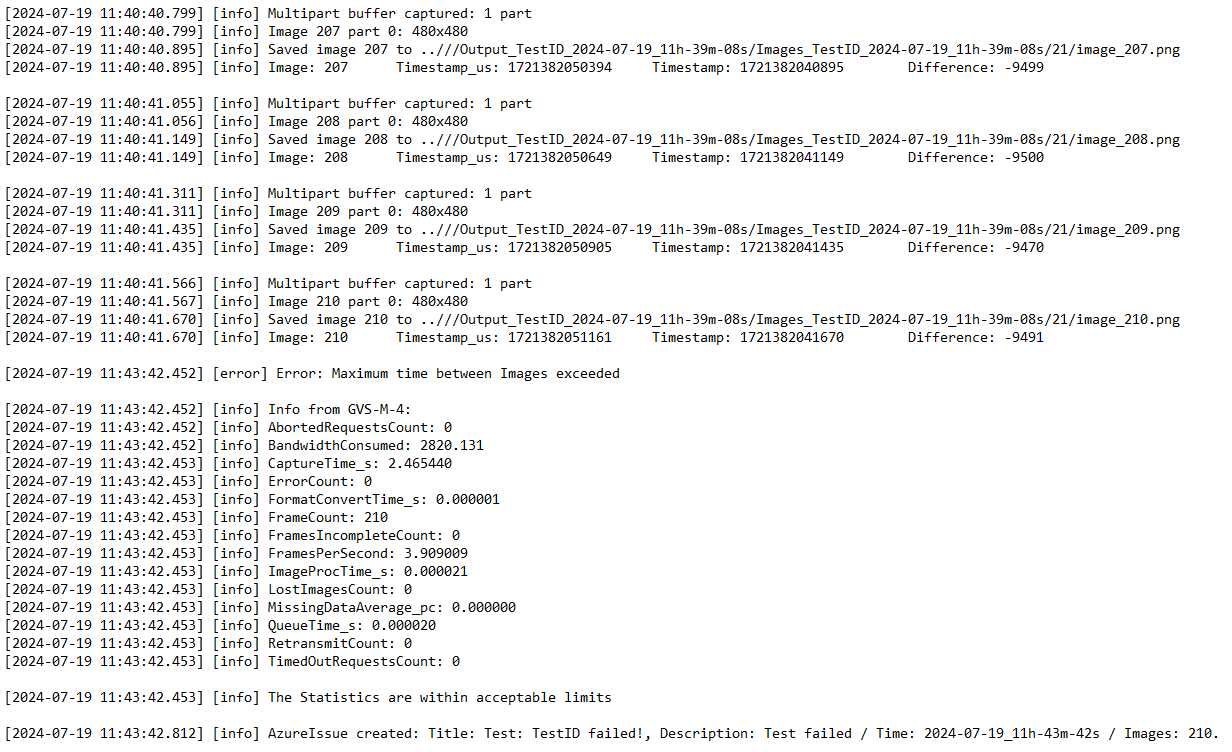
\includegraphics [width=0.9\textwidth]{Logfile.png}
    \caption[Beispiel Log-Datei]{Beispiel Log-Datei (eigene Darstellung)}
    \label{fig:Logfile}
\end{figure}

Um die Performance des Systems nicht zu beeinträchtigen und das Handling der Log-Dateien zu vereinfachen, wird eine Log-Rotation implementiert. Hierbei werden Parameter für die 
maximale Größe einer Log-Datei und die maximale Anzahl an Log-Dateien festgelegt. Der Benutzer kann damit individuell einstellen, wie weit die Informationen der Log-Dateien 
zurückgehen sollen. Eine Archivierung älterer Log-Dateien wird nicht umgesetzt, da der Benutzer bei Bedarf eine entsprechend hohe Anzahl an maximalen Log-Dateien einstellen kann.

Es wird synchrones Logging eingesetzt, da auf die korrekte Reihenfolge und die Vollständigkeit der Logs großer Wert gelegt wird. Zudem ist die Performance des 
Testprogramms nicht in einem solchen Grad entscheidend, dass eine andere Lösung notwendig ist. Durch synchrones Logging bleibt der Quellcode des Testprogramms einfach lesbar und 
es ist nachvollziehbar, an welcher Stelle die jeweilige Log-Nachricht entsteht.

Bei bestimmten Fehlern oder dem erzwungenen Abbruch des Testprogramms wird ein \glqq Azure Issue\grqq\ erstellt, um den Benutzer über das Ereignis zu informieren. Dies ist notwendig, da der 
Benutzer nicht ständig am Testaufbau anwesend ist und Langzeittests auch außerhalb der Arbeitszeit laufen. Diese Funktion arbeitet unabhängig von der Erstellung der Log-Dateien, um 
verzichtbare Abhängigkeiten zu vermeiden.

Um eine klare Trennung der Informationen des Testdurchlaufs von denen des Testprogramms sicherzustellen, werden die Informationen und gegebenenfalls Fehlermeldungen des Testprogramms 
im Terminal ausgegeben. Dies ist sinnvoll, da das Testprogramm direkt nach dem Start die meisten Funktionen durchläuft und anschließend hauptsächlich sich wiederholende 
Abschnitte ausführt. Der Benutzer ist beim Start des Tests in der Regel am Aufbau anwesend und kann daher falls notwendig eingreifen. Für den Fall, dass der Benutzer nicht 
anwesend ist und um die Informationen zusätzlich konsistent zu speichern, wird neben den Log-Dateien für die Datenverarbeitung eine zusätzliche Log-Datei speziell für die 
Überwachung der Funktionen des Testprogramms erstellt. Diese Log-Datei verwendet dieselbe Formatierung wie die anderen Log-Dateien, ist jedoch eine einfache, nicht konfigurierbare 
Datei mit einem festgelegten Log-Level. Dies ist ausreichend, da das Testprogramm nur einen abschätzbaren, begrenzten Umfang an Log-Nachrichten liefert. Außerdem wird dadurch 
vermieden, dass es bei der Konfiguration des Tests durch zu viele Parameter zu Verwirrungen kommt.

Für die Implementierung des Loggings in C++ wird die Bibliothek \glqq spdlog\grqq\ verwendet. Diese ermöglicht eine einfache Konfiguration inklusive des Log-Levels, 
der Formatierung der Log-Nachrichten und der Log-Rotation. Die manuelle Implementierung dieser Eigenschaften über standardmäßige Dateioperationen ist sehr aufwendig und schränkt 
die Flexibilität bei der Konfiguration der Features (z.B. der Log-Rotation) ein. Die Bibliothek \glqq spdlog\grqq\ wird verwendet, da sie eine umfassende Dokumentation 
bietet, benutzerfreundlich ist und viele Konfigurationsmöglichkeiten erlaubt.
	\chapter{Implementierung des Testkonzepts in C++}
\section{Aufbau und Organisation des Projektordners}

\begin{figure}[htbp]
    \centering
      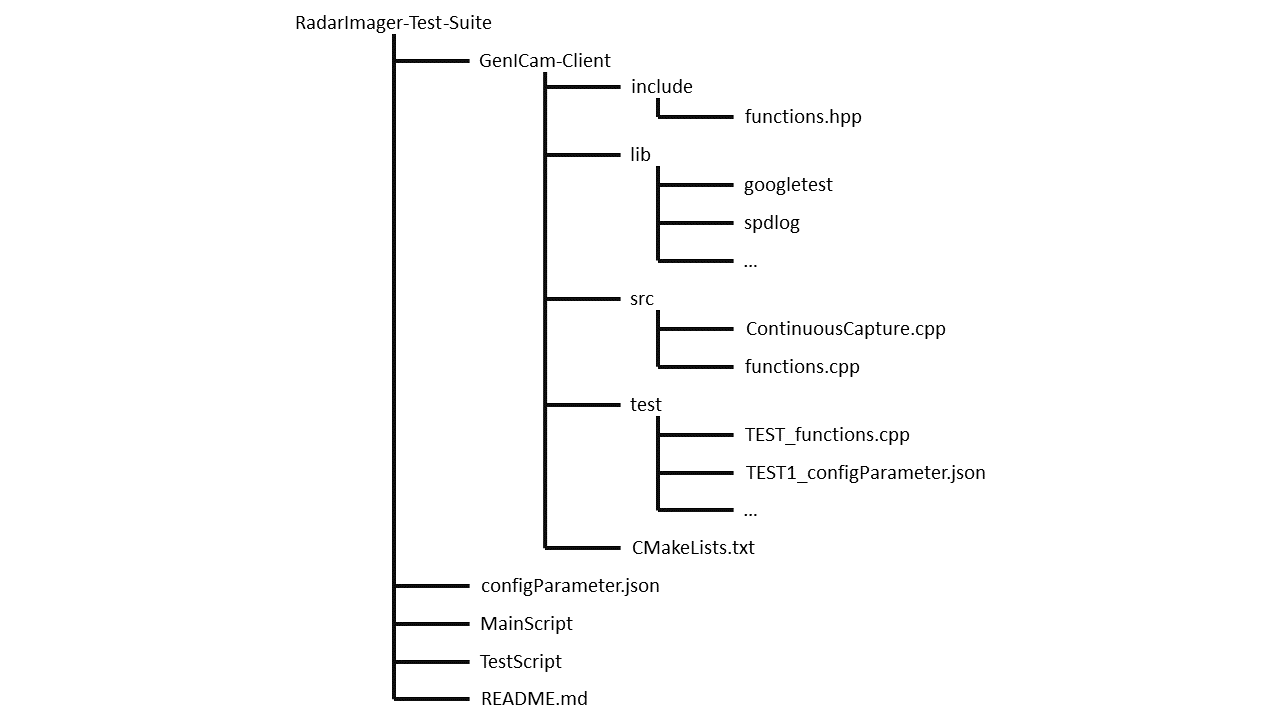
\includegraphics [width=1\textwidth]{Projektstruktur.png}
    \caption[Verzeichnisstruktur]{Verzeichnisstruktur (eigene Darstellung)}
    \label{fig:Verzeichnisstruktur}
\end{figure}

Die Struktur des Testprogramms für den RadarImager ist durch mehrere Unterverzeichnisse klar und logisch aufgebaut. Im Rahmen dieser Projektarbeit liegt der Fokus auf dem 
Verzeichnis \glqq GenICam-Client\grqq. Die Konfigurationsdatei \glqq configParameter.json\grqq\ befindet sich im Hauptordner des Projekts, da sie codeübergreifend 
verwendet wird. Die Ordner \glqq MainScript\grqq\ und \glqq TestScript\grqq, die unter anderem Python-Skripte zur Steuerung des Hardware-Triggers enthalten, sind für diese Arbeit 
von untergeordneter Bedeutung.

Die Codebasis des GenICam-Clients ist zur besseren Übersicht und Handhabbarkeit in folgende Unterverzeichnisse aufgeteilt:

\begin{itemize}
    \item \textbf{include}: Dieser Ordner enthält die Header-Datei \glqq functions.hpp\grqq, welche die Schnittstellen für die in \glqq src\grqq\ implementierten Klassen und Funktionen deklariert. Zudem sind hier verschiedene Strukturen (structs) definiert.
    \item \textbf{lib}: Hier sind die im Projekt verwendeten Bibliotheken, wie zum Beispiel \glqq spdlog\grqq, abgelegt. Diese Strukturierung unterstützt eine klare Abgrenzung zwischen eigenem Code und externen Bibliotheken.
    \item \textbf{src}: Dieser Ordner enthält den Quellcode des Projekts, einschließlich der Hilfsfunktionen und dem Hauptprogramm zur Verarbeitung der empfangenen Daten.
    \item \textbf{test}: In diesem Verzeichnis befinden sich die Modultests, die zur Überprüfung der Funktionalität des Codes dienen. Es umfasst auch zusätzliche Dateien, die in den Tests verwendet werden.
\end{itemize}

Zur Automatisierung und effizienten Verwaltung des Build-Prozesses wird CMake eingesetzt. CMake erleichtert die Integration und Verwaltung von Abhängigkeiten sowie 
die Konfiguration des Testframeworks, um eine konsistente und fehlerfreie Build-Umgebung zu gewährleisten. Hierzu wird eine CMakeLists.txt-Datei angelegt. 
Diese Datei enthält spezifische Anweisungen, die es CMake ermöglichen, die notwendigen Bibliotheken korrekt zu lokalisieren, einzubinden und mit dem Hauptprojekt zu verknüpfen. 
Dadurch wird sichergestellt, dass alle Komponenten des Projekts nahtlos zusammenarbeiten und die Build-Prozesse reibungslos ablaufen können.

Im Anhang dieser Projektarbeit finden sich die Quellcodedateien \glqq ContinuousCapture.cpp\grqq, \glqq functions.hpp\grqq\ und \glqq functions.cpp\grqq.
\section{Verarbeitung der Konfigurationsdatei} \label{Konfigurationsdatei}

Um die Parameter aus der Konfigurationsdatei effektiv im Code zu nutzen, empfiehlt es sich, diese zunächst in Variablen zu speichern. Hierfür wird eine Struktur angelegt, die 
sowohl die vom Benutzer festgelegten Werte als auch daraus resultierende Werte enthält. Bevor die Parameter aus der JSON-Datei in die Variablen übernommen werden, ist eine 
Überprüfung der Datentypen notwendig. Dies verhindert unerwünschte implizite Datentypkonvertierungen und Fehler. Die Verarbeitung der JSON-Datei erfolgt mithilfe der 
\glqq nlohmann/json\grqq-Bibliothek, die eine robuste und effiziente Handhabung von JSON-Daten ermöglicht.

\vspace{6pt}

\begin{lstlisting}[
    caption={Parsen der JSON-Datei},
    label={lst:JSON-Parse},
    language=C++,
    style=myCPP,
    basicstyle=\small\ttfamily,
    numberstyle=\small
]
ifstream paramFile(configFilename);
nlohmann::json root;
paramFile >> root;
\end{lstlisting}

Zunächst wird ein Input-File-Stream-Objekt erstellt, um die Konfigurationsdatei zu öffnen. Anschließend wird eine Variable \glqq root\grqq\ definiert, die als Container für 
die JSON-Daten dient. Der Inhalt von \glqq paramFile\grqq\ wird in die Variable \glqq root\grqq\ geparsed. Dadurch wird der Inhalt der JSON-Datei in eine strukturierte Form 
umgewandelt, die programmatisch einfacher zu verarbeiten ist. Dann kann der Datentyp eines Parameters überprüft werden:

\vspace{12pt}

\begin{lstlisting}[
    caption={Überprüfung des Datentyps},
    label={lst:Datentyp-Test},
    language=C++,
    style=myCPP,
    basicstyle=\small\ttfamily,
    numberstyle=\small
]
root["Basic"]["testID"].is_string()
\end{lstlisting}

Mithilfe der eckigen Klammern wird durch die Struktur der JSON-Datei navigiert. Die Methode \glqq is\_string()\grqq\ überprüft, ob der Wert an der angegebenen Stelle vom Typ
\glqq string\grqq\ ist. Falls einer der Datentypen inkorrekt ist, wird eine Fehlermeldung ausgegeben und das Testprogramm abgebrochen. Sind alle Datentypen korrekt, werden 
die Parameter in die vorgesehene Struktur übertragen. Hierbei ist \glqq param\grqq\ eine Instanz der Struktur für die Parameter (siehe Anhang: Seite \pageref{ParamStruct} ab Zeile 32).

\vspace{12pt}

\begin{lstlisting}[
    caption={Übernahme der Parameter},
    label={lst:Parameter-Übernahme},
    language=C++,
    style=myCPP,
    basicstyle=\small\ttfamily,
    numberstyle=\small
]
param.testID = root["Basic"]["testID"];
\end{lstlisting}

Anschließend erfolgt eine Plausibilitätsprüfung der Parameter. Dabei wird beispielsweise überprüft, dass eingegebene Strings nicht leer sind oder Pfade nur zulässige Zeichen 
enthalten. Bei numerischen Werten wird kontrolliert, ob diese im zugelassenen Bereich liegen, wie etwa beim Log-Level, das nur vier Werte (0 bis 3) zulässt.

Nach erfolgreicher Überprüfung werden der Ausgabeordner und die zugehörigen Unterverzeichnisse erstellt, die zur besseren Nachverfolgbarkeit einen Zeitstempel im Namen enthalten. Außerdem
wird dadurch vermieden, dass einer der Ordner unabsichtlich überschrieben wird.
Die Klasse \glqq TimestampProvider\grqq\ generiert diesen Zeitstempel, wobei zwischen sekunden- und millisekundengenauer Genauigkeit gewählt werden kann (siehe Anhang: Seite \pageref{TimestampProvider1} ab Zeile 66 und \pageref{TimestampProvider2} ab Zeile 5). Bei Problemen während des 
Erstellens der Ordner wird eine Fehlermeldung ausgegeben und in die Log-Datei für das Testprogramm geschrieben.

Die Methoden und Konstanten für die Parameterbereiche sind in der Klasse \glqq ConfigurationHandler\grqq\ abgelegt (siehe Anhang: Seite \pageref{ConfigurationHandler} ab Zeile 79). Dies fördert die Kapselung von Daten und bietet eine klare 
Schnittstelle durch eine Hauptmethode, die interne Methoden aufruft und so die Funktionalität zentral verwaltet.
\section{Umsetzung der Konfigurationsmöglichkeiten}

Die Implementierung der verschiedenen Konfigurationsmöglichkeiten für die Speicherung von Bildern oder Bildstapeln wird in der Callback-Funktion \glqq processRequest\grqq\
sowie in den zugehörigen Hilfsfunktionen der Klasse \glqq ImageSavePreparer\grqq\ (siehe Anhang: Seite \pageref{processRequest} ab Zeile 6, \pageref{ImageSavePreparer1} ab Zeile 106 und \pageref{ImageSavePreparer2} ab Zeile 246) realisiert. Bei Empfang eines Bildes oder Bildstapels prüft die Funktion zunächst, ob eine 
Speicherung gemäß der aktuellen Konfigurationseinstellungen erforderlich ist.

Anschließend wird unterschieden, ob es sich um ein einzelnes Bild oder um einen Bildstapel handelt. Diese Unterscheidung basiert auf der Anzahl der Bilder (Parts), die der 
empfangene Container enthält. Der Speichervorgang variiert je nachdem, ob ein einzelnes Bild oder ein Bildstapel vorliegt. Listing \ref{lst:save} zeigt diese Differenzierung 
und den Ablauf des Speichervorgangs:

\vspace{12pt}

\begin{lstlisting}[
    caption={Speichervorgang},
    label={lst:save},
    language=C++,
    style=myCPP
]
@\textcolor{CommentGreen}{// Save images depending on the configuration}@
@\textcolor{KeywordPurple}{if}@ (@\textcolor{black}{param}@.@\textcolor{black}{saveImages}@ && (@\textcolor{black}{param}@.@\textcolor{black}{saveImagesInterval}@ == 1 || @\textcolor{black}{pRequest}@->@\textcolor{black}{infoFrameID}@.@\textcolor{FunctionsYellow}{read}@() % @\textcolor{black}{param}@.@\textcolor{black}{saveImagesInterval}@ == 1))
{
  @\textcolor{KeywordPurple}{if}@ (@\textcolor{black}{bufferPartCount}@ == 1)  @\textcolor{CommentGreen}{// Buffer has exactly one image}@
  {
    @\textcolor{TypeBlue}{int}@ @\textcolor{black}{imageNumber}@ = @\textcolor{FunctionsYellow}{ceil}@((@\textcolor{TypeBlue}{float}@)@\textcolor{black}{pRequest}@->@\textcolor{black}{infoFrameID}@.@\textcolor{FunctionsYellow}{read}@()/(@\textcolor{TypeBlue}{float}@)@\textcolor{black}{param}@.@\textcolor{black}{saveImagesInterval}@);
    @\textcolor{TypeBlue}{string}@ @\textcolor{black}{filename}@ = @\textcolor{black}{save}@.@\textcolor{FunctionsYellow}{prepareImageSave}@(@\textcolor{black}{param}@, @\textcolor{black}{imageNumber}@);
    @\textcolor{black}{pRequest}@->@\textcolor{FunctionsYellow}{getBufferPart}@(0).@\textcolor{FunctionsYellow}{getImageBufferDesc}@().@\textcolor{FunctionsYellow}{save}@(@\textcolor{black}{filename}@);
    @\textcolor{black}{loggerClient}@->@\textcolor{FunctionsYellow}{info}@("@\textcolor{StringOrange}{Saved image \{\} to \{\}}@", @\textcolor{black}{pRequest}@->@\textcolor{black}{infoFrameID}@.@\textcolor{FunctionsYellow}{read}@(), @\textcolor{black}{filename}@);
  }
  @\textcolor{KeywordPurple}{else}@  @\textcolor{CommentGreen}{// Buffer has more than one image}@
  {
    @\textcolor{TypeBlue}{string}@ @\textcolor{black}{filename}@ = @\textcolor{black}{save}@.@\textcolor{FunctionsYellow}{prepareBufferSave}@(@\textcolor{black}{param}@, @\textcolor{black}{pRequest}@->@\textcolor{black}{infoFrameID}@.@\textcolor{FunctionsYellow}{read}@(), @\textcolor{black}{i}@);
    @\textcolor{black}{pRequest}@->@\textcolor{FunctionsYellow}{getBufferPart}@(@\textcolor{black}{i}@).@\textcolor{FunctionsYellow}{getImageBufferDesc}@.@\textcolor{FunctionsYellow}{save}@(@\textcolor{black}{filename}@);
    @\textcolor{black}{loggerClient}@->@\textcolor{FunctionsYellow}{info}@("@\textcolor{StringOrange}{Saved image \{\} part \{\} to \{\}}@", @\textcolor{black}{pRequest}@->@\textcolor{black}{infoFrameID}@.@\textcolor{FunctionsYellow}{read}@(), @\textcolor{black}{i}@, @\textcolor{black}{filename}@);
  }
}
\end{lstlisting}

\paragraph{Einzelbild}

Um die Nummer des aktuell zu speichernden Bildes zu bestimmen, wird die Identifikationsnummer des Bildes durch das festgelegte Speicherintervall geteilt. Diese Nummer 
wird für die Vorbereitung des Speichervorgangs verwendet. In diesem Schritt wird der Pfad zum Speicherort generiert und bei Bedarf ein neuer
Ordner angelegt. Hierbei wird zwischen der Nummerierung der Ordner und der Benennung mittels eines Zeitstempels unterschieden.

Bei Nummerierung setzt sich der Pfad aus dem Hauptverzeichnis für Bilder und einem Unterverzeichnis, das die aktuelle Ordner-Nummer trägt, zusammen. Erreicht das Speicherintervall 
den Punkt, an dem ein neuer Ordner benötigt wird, wird dieser mit der entsprechenden Nummer erstellt. Im Falle der Benennung durch einen Zeitstempel erhalten die Unterverzeichnisse 
Namen, die den Zeitstempel bis auf Millisekunden genau wiedergeben. Die Benennung auf die Millisekunde genau ist notwendig, um das unabsichtliche Überschreiben der Verzeichnisse zu verhindern, da je nach Konfiguration 
mehrere Verzeichnisse pro Sekunde erstellt werden. Es ist dabei zusätzlich erforderlich, den Namen des aktuellen oder vorherigen Ordners zu speichern, da der Zeitstempel nicht 
einfach rekonstruiert werden kann für die nächsten Bilder, die im selben Ordner abgelegt werden sollen.

Nachdem Erstellen des Pfads und gegebenenfalls dem Anlegen eines neuen Ordners, übergibt die Untermethode \glqq createImageSubpathFolder\grqq\ den Pfad an die Methode \glqq prepareImageSave\grqq\ (siehe Anhang: Seite \pageref{ImageSavePreparer2} ab Zeile 246). 
Diese ist verantwortlich für die Erstellung des Bildnamens und somit für die Festlegung des endgültigen Speicherorts des Bildes. Auch hier wird zwischen Nummerierung und Zeitstempel 
differenziert.

Schließlich wird das Bild am festgelegten Speicherort durch den Aufruf der \glqq save\grqq-Methode des Impact Acquire SDK gespeichert.

\paragraph{Bildstapel}

Bei der Verarbeitung eines Bildstapels erfolgt die Vorbereitung ähnlich wie bei Einzelbildern, allerdings wird für jeden Container ein neuer Ordner angelegt. Innerhalb einer 
for-Schleife, in der auch der Code aus Listing \ref{lst:save} implementiert ist, wird die Hilfsvariable \glqq i\grqq\ inkrementiert, die das aktuelle Bild im Stapel kennzeichnet. 
Ein neuer Ordner wird immer dann erstellt, wenn \glqq i\grqq\ den Wert 0 annimmt, der das erste Bild eines neuen Bildstapels signalisiert.

Die Methode \glqq prepareBufferSave\grqq\ ist anschließend dafür zuständig, den Namen der Bilddatei zu bestimmen (siehe Anhang: Seite \pageref{prepareBufferSave} ab Zeile 335). Abhängig von der Konfiguration wird hierbei entweder die Nummer des 
Bildes innerhalb des Stapels (\glqq i\grqq) oder ein Zeitstempel verwendet. In jedem Fall wird die Nummer des Containers in die Benennung der Datei integriert.

Das aktuelle Bild wird dann am vorbereiteten Speicherort abgelegt. Dieser Prozess wiederholt sich durch die for-Schleife für jedes Bild des Stapels.
\section{Umsetzung des Loggings} \label{Logging}

Um einen Logger mithilfe der Bibliothek \glqq spdlog\grqq\ zu implementieren, ist zunächst eine Initialisierung erforderlich. Diese erfolgt über eine Methode, die abhängig von 
den übergebenen Parametern eine Log-Rotation mit definierter maximaler Dateigröße und Anzahl an Dateien erstellt (siehe Anhang: Seite \pageref{initializeLogger} ab Zeile 395). 
Zusätzlich wird das Log-Level durch eine Hilfsfunktion festgelegt (siehe Anhang: Seite \pageref{setLogLevel} ab Zeile 356).

Nach der Initialisierung kann der Logger in Funktionen und Methoden eingebunden werden. Dies geschieht durch folgenden Aufruf:

\vspace{12pt}

\begin{lstlisting}[
    caption={Aufruf des Loggers},
    label={lst:logAufruf},
    language=C++,
    style=myCPP,
    basicstyle=\small\ttfamily,
    numberstyle=\small
]
auto loggerClient = spdlog::get("logClient");
\end{lstlisting}

Innerhalb der Callback-Funktion \glqq processRequest\grqq\ werden relevante Informationen zur Datenübertragung protokolliert. Es wird vermerkt, wenn ein Bildstapel empfangen wird, 
einschließlich der Anzahl der enthaltenen Bilder und der Größe jedes einzelnen Bildes. Auch nach erfolgreichem Speichern eines Bildes wird eine entsprechende Log-Nachricht erstellt. 
Zudem werden die Zeiten für die Erstellung und Speicherung der Bilder sowie deren Differenz dokumentiert. Treten Fehler auf, so werden diese ebenfalls sorgfältig festgehalten. Ein 
typisches Beispiel für einen solchen Fehler ist der Empfang eines Bildes außerhalb des vorgesehenen Containers. Dies deutet auf eine Fehlfunktion des RadarImagers hin, da unter 
regulären Bedingungen jedes Bild innerhalb eines Containers übermittelt wird.

Regelmäßig werden wichtige Statistiken wie \ac{FPS}, Frame Count und die Anzahl verlorener Bilder in die Log-Dateien geschrieben. Diese Daten werden über das Impact 
Acquire \acs{SDK} bezogen und auf Auffälligkeiten hin überprüft. Bei signifikanten Änderungen der \ac{FPS} oder einer Zunahme verlorener Bilder im Vergleich zur letzten Überprüfung 
wird eine Warnung ausgegeben, um im Nachinein mögliche Probleme identifizieren zu können. Dies ist besonders relevant, wenn ein Fehler zum Abbruch des Tests führt, beispielsweise 
bei einer fehlerhaften Anfrage.

Zum Monitoring wird die \glqq cURL\grqq-Bibliothek genutzt, um über eine HTTP-Anfrage ein \glqq Azure Issue\grqq\ zu erstellen. Die Methode \glqq createAzureIssue\grqq\
in der Klasse \glqq AzureIssueCreator\grqq\ sendet eine HTTP POST-Anfrage an die Azure DevOps REST-API, um ein \glqq Azure Issue\grqq\ mit spezifischen Feldern wie Titel, 
Beschreibung und zugewiesenem Benutzer zu erstellen (siehe Anhang: Seite \pageref{AzureIssueCreator1} ab Zeile 146 und \pageref{AzureIssueCreator2} ab Zeile 502). Die Authentifizierung erfolgt über ein in \glqq Base64\grqq\ kodiertes \ac{PAT}. Die Serverantwort wird protokolliert und 
relevante Informationen werden in die Log-Dateien geschrieben.

Um das Testprogramm automatisch zu beenden, falls über einen längeren Zeitraum keine Bilder empfangen werden, überwacht eine while-Schleife im Hauptprogramm die Zeit seit der letzten 
Anfrage. Diese Schleife endet entweder durch Überschreitung dieser Zeitgrenze oder durch das Drücken einer Taste (siehe Anhang: Seite \pageref{while-Schleife} ab Zeile 155). Eine Hilfsfunktion ermöglicht dabei die parallele Abfrage der 
Tastatureingabe.

Zusätzlich zum Logging der Datenübertragung und Speicherung wird die separate Log-Datei zur Überwachung des korrekten Ablaufs des Testprogramms geführt. Diese Log-Datei wird unabhängig 
von den Hilfsfunktionen für das Logging verwaltet, um auch dort mögliche Fehlerquellen zu identifizieren.
\section{Entwicklung und Durchführung der Modultests}

Um die Funktionalität und Zuverlässigkeit des Testprogramms zu gewährleisten, werden umfassende Modultests mit dem Testframework \glqq googletest\grqq\ durchgeführt. Für jede Klasse des 
Produktivcodes wird eine entsprechende Testklasse erstellt. Diese Testklassen erben von \glqq ::testing::Test\grqq\ und ermöglichen die Definition von Setup- und Teardown-Methoden, 
die jeweils vor und nach den Testfällen ausgeführt werden. Diese Methoden ermöglichen die Initialisierung und Bereinigung der Testumgebung. Somit wird eine konsistente Ausführung 
der Tests sicherstellt.

Ein spezielles Beispiel der Modultests ist der Test der Klasse \glqq ConfigurationHandler\grqq. In diesem Test werden verschiedene Muster-Konfigurationsdateien verwendet, um 
unterschiedliche Szenarien zu simulieren. Diese Dateien umfassen sowohl korrekte Konfigurationen als auch solche mit inkorrekten Datentypen oder Werten, die außerhalb des zulässigen 
Bereichs liegen. Listing \ref{lst:AuszugModultests} zeigt exemplarisch jeweils einen Modultest für diese Fälle:

\vspace{12pt}

\begin{lstlisting}[
    caption={Beispiel Modultests},
    label={lst:AuszugModultests},
    language=C++,
    style=myCPP
]
@\textcolor{FunctionsYellow}{TEST\_F}@(@\textcolor{ClassGreen}{ConfigurationHandlerTest}@, ValidConfigA)
{
  @\textcolor{black}{config}@.@\textcolor{black}{configFilename}@ = "../test/TEST1_configParameter.json";
  @\textcolor{FunctionsYellow}{EXPECT\_TRUE}@(@\textcolor{black}{config}@.@\textcolor{FunctionsYellow}{loadConfiguration}@(param));

  @\textcolor{FunctionsYellow}{EXPECT\_EQ}@(@\textcolor{black}{param}@.@\textcolor{black}{saveImages}@, true);
  @\textcolor{FunctionsYellow}{EXPECT\_EQ}@(@\textcolor{black}{param}@.@\textcolor{black}{numberImages}@, true);
  @\textcolor{FunctionsYellow}{EXPECT\_EQ}@(@\textcolor{black}{param}@.@\textcolor{black}{numberFolders}@, true);
  @\textcolor{FunctionsYellow}{EXPECT\_EQ}@(@\textcolor{black}{param}@.@\textcolor{black}{saveImagesInterval}@, 1);
  @\textcolor{FunctionsYellow}{EXPECT\_EQ}@(@\textcolor{black}{param}@.@\textcolor{black}{newFolderInterval}@, 10);
  @\textcolor{FunctionsYellow}{EXPECT\_EQ}@(@\textcolor{black}{param}@.@\textcolor{black}{createLog}@@\textcolor{black}{param.createLog}@, true);
  @\textcolor{FunctionsYellow}{EXPECT\_EQ}@(@\textcolor{black}{param}@.@\textcolor{black}{logLevel}@, 1);
  @\textcolor{FunctionsYellow}{EXPECT\_EQ}@(@\textcolor{black}{param}@.@\textcolor{black}{maxLogFiles}@, 3);
  @\textcolor{FunctionsYellow}{EXPECT\_EQ}@(@\textcolor{black}{param}@.@\textcolor{black}{maxLogSize}@, 5);
  @\textcolor{FunctionsYellow}{EXPECT\_EQ}@(@\textcolor{black}{param}@.@\textcolor{black}{createIssue}@, true);
  @\textcolor{FunctionsYellow}{EXPECT\_EQ}@(@\textcolor{black}{param}@.@\textcolor{black}{testID}@, "TestID");

  @\textcolor{FunctionsYellow}{EXPECT\_TRUE}@(@\textcolor{ClassGreen}{filesystem}@::@\textcolor{FunctionsYellow}{exists}@(@\textcolor{black}{param}@.@\textcolor{black}{outputPath}@));
  @\textcolor{FunctionsYellow}{EXPECT\_TRUE}@(@\textcolor{ClassGreen}{filesystem}@::@\textcolor{FunctionsYellow}{exists}@(@\textcolor{black}{param}@.@\textcolor{black}{imagesPath}@));
  @\textcolor{FunctionsYellow}{EXPECT\_TRUE}@(@\textcolor{ClassGreen}{filesystem}@::@\textcolor{FunctionsYellow}{exists}@(@\textcolor{black}{param}@.@\textcolor{black}{logsPath}@));

  @\textcolor{ClassGreen}{filesystem}@::@\textcolor{FunctionsYellow}{remove\_all}@(@\textcolor{black}{param}@.@\textcolor{black}{outputPath}@);
}

@\textcolor{FunctionsYellow}{TEST\_F}@(@\textcolor{ClassGreen}{ConfigurationHandlerTest}@, InvalidDatatypeBool)
{
  @\textcolor{black}{config}@.@\textcolor{black}{configFilename}@ = "../test/TEST3_configParameter.json";
  @\textcolor{FunctionsYellow}{EXPECT\_FALSE}@(@\textcolor{black}{config}@.@\textcolor{FunctionsYellow}{loadConfiguration}@(param));
}
\end{lstlisting}

Mithilfe der gültigen Muster-Konfigurationsdateien wird die korrekte Übernahme der in den Konfigurationsdateien festgelegten Werte in die entsprechenden Variablen überprüft. 
Ungültige Konfigurationsdateien dienen dazu, die Fähigkeit des Testprogramms zu validieren, Fehler zu erkennen und zu melden, um einen fehlerhaften Betrieb zu verhindern.

Ein Aspekt der Testimplementierung ist das Mocking externer Abhängigkeiten, um eine Isolation der Tests zu gewährleisten. Durch das Ersetzen realer Abhängigkeiten mit Mock-Objekten 
können Tests in einer kontrollierten Umgebung durchgeführt werden. Die Mock-Objekte simulieren dabei ein für den jeweiligen Modultest festgelegtes Verhalten der Abhängigkeiten.
Dies ist insbesondere für das Testen von Komponenten, die mit externen Systemen interagieren, von großer Bedeutung.

Für eine zuverlässige Überprüfung der Methode \glqq checkKeyboardHit\grqq\ (siehe Anhang: Seite \pageref{checkKeyboardHit} ab Zeile 618) ist es notwendig Systemaufrufe zu simulieren. Hierfür werden mittels Mocking verschiedene Systemaufrufe 
angepasst. Dies ermöglicht es, das Verhalten der Tastatureingabe ohne tatsächliche Benutzerinteraktion zu testen. Dafür sind Funktionen notwendig, die Standardbibliothekfunktionen
durch die gemockten Funktionen ersetzen.

Durch die Abdeckung jeder Klasse des Testprogramms mit Modultests wird eine hohe Sicherheit des Testablaufs gewährleistet. Aktuell existieren jedoch keine Modultests für die 
Callback-Funktion und die Hauptfunktion. Die Herausforderung besteht darin, dass durch die Nutzung des Impact Acquire \acs{SDK} zahlreiche Abhängigkeiten zu Klassen und Methoden 
bestehen, die potenziell gemockt werden müssen. Der Aufwand hierfür ist für ein solches Testprogramm unverhältnismäßig hoch. Dennoch decken die bestehenden Modultests viele 
potenzielle Fehlerquellen innerhalb der Callback-Funktion auf, beispielsweise durch Tests der Methoden zur Vorbereitung des Speicherns. Zusätzlich bietet das Impact Acquire \acs{SDK} 
selbst ein umfangreiches Fehlermanagement, das Fehlermeldungen an das Testprogramm weiterleitet.

Die Integration des Testframeworks mittels CMake erleichtert die Ausführung der Modultests erheblich. Nach dem Start der ausführbaren Testdatei wird im Terminal eine 
Übersicht der Tests sowie die Ergebnisse der einzelnen Modultests angezeigt:

\begin{figure}[htbp]
    \centering
      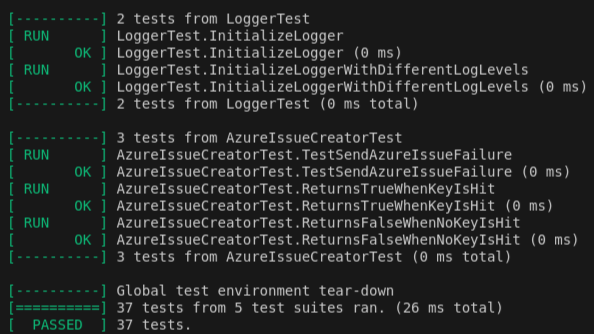
\includegraphics [width=0.75\textwidth]{ErgebnisModultests.png}
    \caption[Ergebnis Modultests]{Ergebnis Modultests (eigene Darstellung)}
    \label{fig:Modultests}
\end{figure}

Neben den Modultests wird das Testprogramm auch regelmäßig durch Verhaltenstests während der Entwicklungsphase überprüft. Somit werden Fehler frühzeitig identifiziert und behoben. 
Obwohl diese Tests die Testabdeckung temporär erhöhen, ist es wichtig zu erwähnen, dass sie nicht als Ersatz für eine systematische und dauerhafte Erweiterung der Testabdeckung durch 
Modultests dienen. Vielmehr ergänzen sie diese, indem sie zusätzliche Sicherheit bieten, dass das Programm auch unter realen Bedingungen zuverlässig funktioniert.
\section{Ablauf des Testprogramms}

Um den Ablauf des Testprogramms nach dem Start eines neuen Tests zu veranschaulichen, werden im Folgenden zwei Flussdiagramme präsentiert. Diese Diagramme skizzieren den 
grundlegenden Ablauf, ohne dabei auf spezifische Details des Quellcodes einzugehen.

\begin{figure}[H]
    \centering
      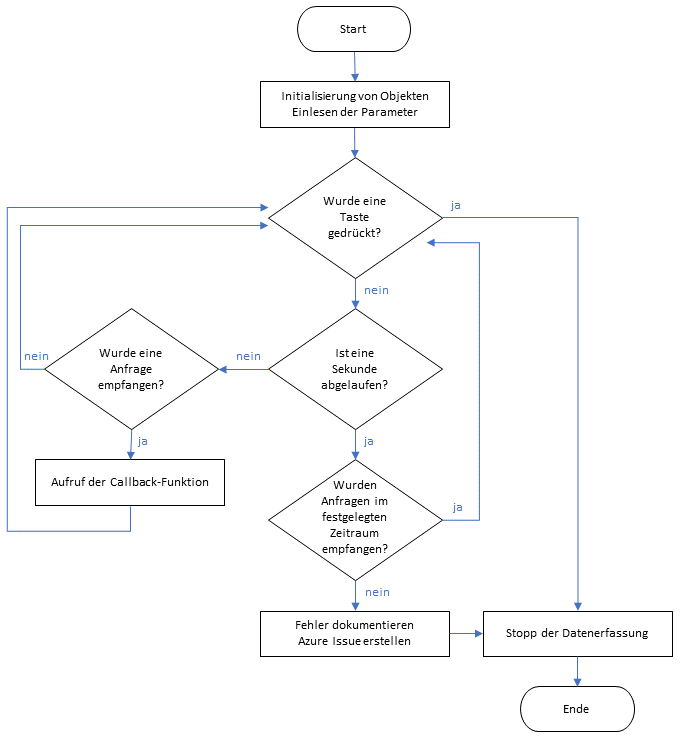
\includegraphics [width=0.68\textwidth]{mainAblauf.png}
    \caption[Flussdiagramm Hauptprogramm]{Flussdiagramm Hauptprogramm (eigene Darstellung)}
    \label{fig:mainAblauf}
\end{figure}

Das Flussdiagramm in Abbildung \ref{fig:mainAblauf} zeigt die Funktionsweise der Hauptfunktion, die zu Beginn des Testprogramms ausgeführt wird. Diese initialisiert am Anfang die benötigten Objekte, die für 
den Zugriff auf die Hilfsfunktionen notwendig sind. Anschließend wird der Logger für die Log-Datei zur Überwachung des Testprogramms erstellt, um den  Prozess nachvollziehen
zu können. Mithilfe der Klasse \glqq ConfigurationHandler\grqq\ wird die Konfiguration eingelesen sowie der Ausgabeordner erstellt (siehe Kapitel \ref{Konfigurationsdatei}). Nach 
erfolgreichem Abschluss dieser Schritte wird der Logger für die Datenübertragung und Speicherung konfiguriert, einschließlich der Festlegung des Log-Levels und der Implementierung 
der Log-Rotation. Diese Schritte setzen das vorherige Einlesen der erforderlichen Parameter voraus, da diese für die Initialisierung erforderlich sind. Im weiteren Verlauf wird das 
Gerät (RadarImager) mittels des Impact Acquire \acs{SDK} initialisiert und für die Kommunikation vorbereitet. Mit diesen Vorbereitungen ist das System bereit, mit der Datenerfassung 
zu beginnen.

Während der Datenerfassung überprüft das Programm kontinuierlich die Kommunikation. Diese Überprüfung erfolgt in einsekündigen Intervallen und stellt sicher, dass innerhalb einer 
festgelegten Zeitspanne Anfragen empfangen werden. Sollte keine Kommunikation feststellbar sein, wird das Programm abgebrochen, eine entsprechende Log-Nachricht erstellt und ein 
\glqq Azure Issue\grqq\ generiert. Solange die Kommunikation ordnungsgemäß funktioniert, bleibt das Programm in Bereitschaft, um Daten zu empfangen und die 
zugehörige Callback-Funktion auszulösen. Dies gewährleistet eine effiziente und kontinuierliche Datenverarbeitung während des Testlaufs.

\begin{figure}[H]
    \centering
      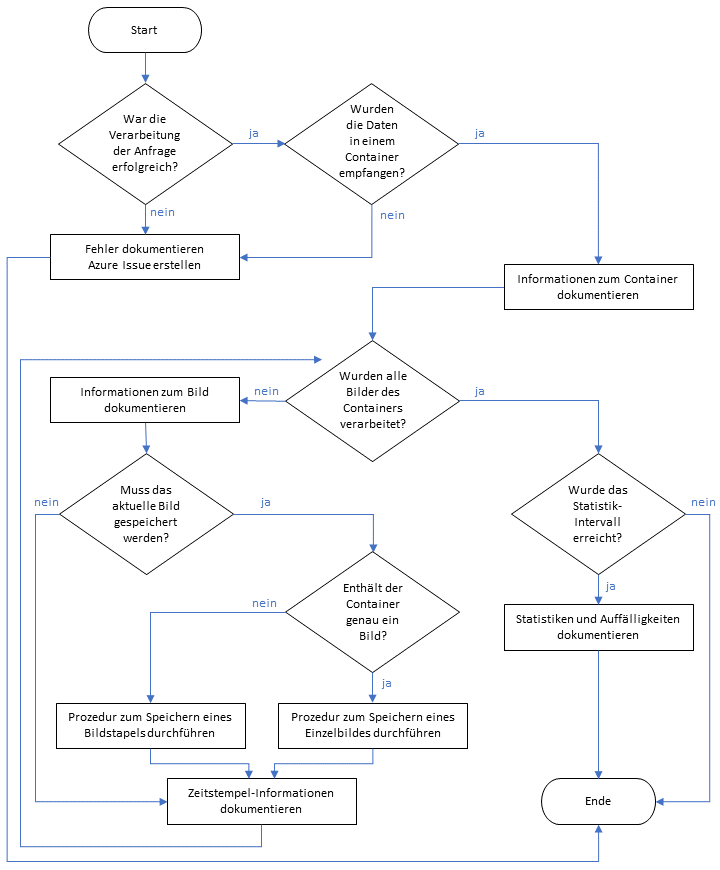
\includegraphics [width=0.7\textwidth]{requestAblauf.png}
    \caption[Flussdiagramm Callback-Funktion]{Flussdiagramm Callback-Funktion (eigene Darstellung)}
    \label{fig:requestAblauf}
\end{figure}

Die Callback-Funktion gliedert sich in zwei Hauptbereiche: Fehlererkennung und Bilddatenverarbeitung (siehe Abbildung \ref{fig:requestAblauf}). Im Bereich der Fehlererkennung werden verschiedene Eigenschaften der empfangenen 
Anfrage auf Kompatibilität mit den erwarteten Werten überprüft. Dies umfasst die Bestätigung, dass die Anfrage erfolgreich verarbeitet ist und die Daten innerhalb eines Containers 
empfangen werden. Ein erkannter Fehler führt zur Protokollierung in einer Log-Nachricht, zur Erstellung eines \glqq Azure Issues\grqq\ und zum Abbruch des Testprogramms.

Im zweiten Bereich, der Bilddatenverarbeitung, werden zunächst Informationen über den empfangenen Container im Terminal dargestellt und in den Log-Dateien vermerkt. Die Verarbeitung 
der Bilder erfolgt durch eine for-Schleife, die durch die Bilder des Containers iteriert. Für jedes Bild werden zusätzliche Informationen ausgegeben und gespeichert. 
Entsprechend den Anforderungen wird gegebenenfalls ein Speichervorgang für das aktuelle Bild initiiert. Unabhängig davon werden der Zeitstempel und die Verarbeitungszeit jedes Bildes 
in den Log-Dateien dokumentiert. Nach der Verarbeitung aller Bilder des Containers werden relevante Statistiken ausgegeben, sobald ein bestimmtes Intervall erreicht ist (siehe Kapitel 
\ref{Logging} und Abbildung \ref{fig:Logfile}). Damit ist die Callback-Funktion abgeschlossen.
	\chapter{Bewertung und Ausblick}

Hier kommt die Bewertung und ein Ausblick
	%\input{content/07kapitel}

	\clearpage
	\pagenumbering{Roman}
	\setcounter{page}{3}	% Seitenzahl anpassen
	
   % Literaturverzeichnis
   \hypersetup{linkcolor=black} 
	\cleardoublepage{}
		\addcontentsline{toc}{chapter}{Literaturverzeichnis}
	\bibliographystyle{dcugerman}
   \literaturverz{T2000_02}
	%\phantomsection \label{listoflit}

	% Glossar
	\printglossary[style=altlist,title=Glossar]

	% Anhang
	\chapter*{Anhang}
\addcontentsline{toc}{chapter}{Anhang}

Hier kommt der Anhang	
	
\end{document}